\documentclass[aspectratio=169]{ctexbeamer}
\setbeamertemplate{bibliography item}{\insertbiblabel}
\usetheme{Madrid}
\beamertemplatenavigationsymbolsempty
\definecolor{tuna}{rgb}{0.098,0.51,0.696}
\definecolor{thu}{rgb}{0.50,0.36,0.71}

\setbeamercolor{section in toc}{fg=black,bg=white}
\setbeamercolor{item}{fg=tuna,bg=white}
\setbeamercolor{alerted text}{fg=tuna!80!gray}
\setbeamercolor*{palette primary}{fg=tuna!60!black,bg=gray!30!white}
\setbeamercolor*{palette secondary}{fg=tuna!70!black,bg=gray!15!white}
\setbeamercolor*{palette tertiary}{bg=tuna!80!black,fg=gray!10!white}
\setbeamercolor*{palette quaternary}{fg=tuna,bg=gray!5!white}

\setbeamercolor*{sidebar}{fg=tuna,bg=gray!15!white}

\setbeamercolor*{palette sidebar primary}{fg=tuna!10!black}
\setbeamercolor*{palette sidebar secondary}{fg=white}
\setbeamercolor*{palette sidebar tertiary}{fg=tuna!50!black}
\setbeamercolor*{palette sidebar quaternary}{fg=gray!10!white}

%\setbeamercolor*{titlelike}{parent=palette primary}
\setbeamercolor{titlelike}{parent=palette primary,fg=tuna}
\setbeamercolor{frametitle}{bg=gray!10!white}
\setbeamercolor{frametitle right}{bg=gray!60!white}

\setbeamercolor*{separation line}{}
\setbeamercolor*{fine separation line}{}

\setbeamertemplate{sections/subsections in toc}[square]
\setbeamertemplate{items}[square]


\usepackage{graphicx}
\usepackage{algpseudocode}
\usepackage{float}
\usepackage{listings}
\usepackage{booktabs}
\usepackage{mathtools}
\usepackage{hyperref}
\usepackage{url}
\usepackage{tikz}
\usetikzlibrary{calc}
\usetikzlibrary{arrows}
\usetikzlibrary{shapes}

\renewcommand{\d}{\mathrm{d}}


\title{Machine Block Placement}
\subtitle{code layout optimizations.}
\author{龙英池}

\AtBeginSection[]{
\begin{frame}
    \vfill
    \centering
    \begin{beamercolorbox}[sep=8pt,center,shadow=true,rounded=true]{title}
        \usebeamerfont{title}\insertsectionhead\par%
    \end{beamercolorbox}
    \vfill
\end{frame}
}

\definecolor{codegreen}{rgb}{0,0.6,0}
\definecolor{codegray}{rgb}{0.5,0.5,0.5}
\definecolor{codepurple}{rgb}{0.58,0,0.82}
\definecolor{backcolour}{rgb}{1,1,1}

\lstdefinelanguage[RISC-V]{Assembler}
{
    alsoletter={.}, % allow dots in keywords
    alsodigit={0x}, % hex numbers are numbers too!
    morekeywords=[1]{ % instructions
            lb, lh, lw, lbu, lhu,
            sb, sh, sw,
            sll, slli, srl, srli, sra, srai,
            add, addi, sub, lui, auipc,
            xor, xori, or, ori, and, andi,
            slt, slti, sltu, sltiu,
            beq, bne, blt, bge, bltu, bgeu,
            j, jr, jal, jalr, ret,
            scall, break, nop
        },
    morekeywords=[2]{ % sections of our code and other directives
            .align, .ascii, .asciiz, .byte, .data, .double, .extern,
            .float, .globl, .half, .kdata, .ktext, .set, .space, .text, .word
        },
    morekeywords=[3]{ % registers
            zero, ra, sp, gp, tp, s0, fp,
            t0, t1, t2, t3, t4, t5, t6,
            s1, s2, s3, s4, s5, s6, s7, s8, s9, s10, s11,
            a0, a1, a2, a3, a4, a5, a6, a7,
            ft0, ft1, ft2, ft3, ft4, ft5, ft6, ft7,
            fs0, fs1, fs2, fs3, fs4, fs5, fs6, fs7, fs8, fs9, fs10, fs11,
            fa0, fa1, fa2, fa3, fa4, fa5, fa6, fa7
        },
    morecomment=[l]{;},   % mark ; as line comment start
    morecomment=[l]{\#},  % as well as # (even though it is unconventional)
    morestring=[b]",      % mark " as string start/end
    morestring=[b]'       % also mark ' as string start/end
}

% usage example:

% define some basic colors
\definecolor{mauve}{rgb}{0.58,0,0.82}

\renewcommand{\lstlistingname}{代码}

\setmonofont{Consolas}

\definecolor{codegreen}{rgb}{0,0.6,0}
\definecolor{codegray}{rgb}{0.5,0.5,0.5}
\definecolor{codepurple}{rgb}{0.58,0,0.82}
\definecolor{backcolour}{rgb}{1,1,1}

\lstdefinelanguage[RISC-V]{Assembler}
{
    alsoletter={.}, % allow dots in keywords
    alsodigit={0x}, % hex numbers are numbers too!
    morekeywords=[1]{ % instructions
            lb, lh, lw, lbu, lhu,
            sb, sh, sw,
            sll, slli, srl, srli, sra, srai,
            add, addi, sub, lui, auipc,
            xor, xori, or, ori, and, andi,
            slt, slti, sltu, sltiu,
            beq, bne, blt, bge, bltu, bgeu,
            j, jr, jal, jalr, ret,
            scall, break, nop
        },
    morekeywords=[2]{ % sections of our code and other directives
            .align, .ascii, .asciiz, .byte, .data, .double, .extern,
            .float, .globl, .half, .kdata, .ktext, .set, .space, .text, .word
        },
    morekeywords=[3]{ % registers
            zero, ra, sp, gp, tp, s0, fp,
            t0, t1, t2, t3, t4, t5, t6,
            s1, s2, s3, s4, s5, s6, s7, s8, s9, s10, s11,
            a0, a1, a2, a3, a4, a5, a6, a7,
            ft0, ft1, ft2, ft3, ft4, ft5, ft6, ft7,
            fs0, fs1, fs2, fs3, fs4, fs5, fs6, fs7, fs8, fs9, fs10, fs11,
            fa0, fa1, fa2, fa3, fa4, fa5, fa6, fa7
        },
    morecomment=[l]{;},   % mark ; as line comment start
    morecomment=[l]{\#},  % as well as # (even though it is unconventional)
    morestring=[b]",      % mark " as string start/end
    morestring=[b]'       % also mark ' as string start/end
}

% usage example:

% define some basic colors
\definecolor{mauve}{rgb}{0.58,0,0.82}

\lstset{
% listings sonderzeichen (for german weirdness)
literate={ö}{{\"o}}1
{ä}{{\"a}}1
{ü}{{\"u}}1,
basicstyle=\tiny\ttfamily,                    % very small code
breaklines=true,                              % break long lines
commentstyle=\itshape\color{green!50!black},  % comments are green
keywordstyle=[1]\color{blue!80!black},        % instructions are blue
keywordstyle=[2]\color{orange!80!black},      % sections/other directives are orange
keywordstyle=[3]\color{red!50!black},         % registers are red
stringstyle=\color{mauve},                    % strings are from the telekom
identifierstyle=\color{teal},                 % user declared addresses are teal
frame=l,                                      % black line on the left side of code
language=[RISC-V]Assembler,                   % all code is RISC-V
tabsize=4,                                    % indent tabs with 4 spaces
showstringspaces=false                        % do not replace spaces with weird underlines
}

\lstdefinestyle{mystyle}{
    backgroundcolor=\color{backcolour},
    commentstyle=\color{codegreen},
    keywordstyle=\color{magenta},
    numberstyle=\tiny\color{codegray},
    stringstyle=\color{codepurple},
    basicstyle=\ttfamily\footnotesize,
    breakatwhitespace=false,
    breaklines=true,
    captionpos=b,
    keepspaces=true,
    numbers=left,
    numbersep=5pt,
    showspaces=false,
    showstringspaces=false,
    showtabs=false,
    tabsize=2
}

\lstset{style=mystyle,language=C++}

\begin{document}
\frame{\titlepage}

\begin{frame}
\frametitle{目录}
\tableofcontents
\end{frame}

\section{代码布局(Code Layout)}

\begin{frame}[fragile]
    \frametitle{什么是代码布局}
    指令连续地、有顺序地储存在内存中。LLVM中,这些优化过程抽象成控制流图中的基本块(Basic Block, BB)的排列方式。

    \begin{columns}
        \begin{column}{0.2\textwidth}
            \centering
            C Codes:
            \begin{lstlisting}
if (a < b)
    c = 1;\end{lstlisting}
        \end{column}
        \begin{column}{0.5\textwidth}
\begin{lstlisting}[language={[RISC-V]Assembler}]
; a is in a0
; b is in a1
; c is in a2
bge a0 a1 .LBB0_2
j .LBB0_1
li a2 1
.LBB0_2:\end{lstlisting}
        \end{column}
    \end{columns}
\end{frame}

\begin{frame}
    \frametitle{机器代码布局优化}
    基于机器相关的,代码布局的优化主要包含,基本块放置(Basic block placement)、基本块对齐(Basic block alignment)、冷热代码分离(Hot-Cold Splitting)\cite{bakhvalov-2019}.
    \begin{figure}
        \centering
        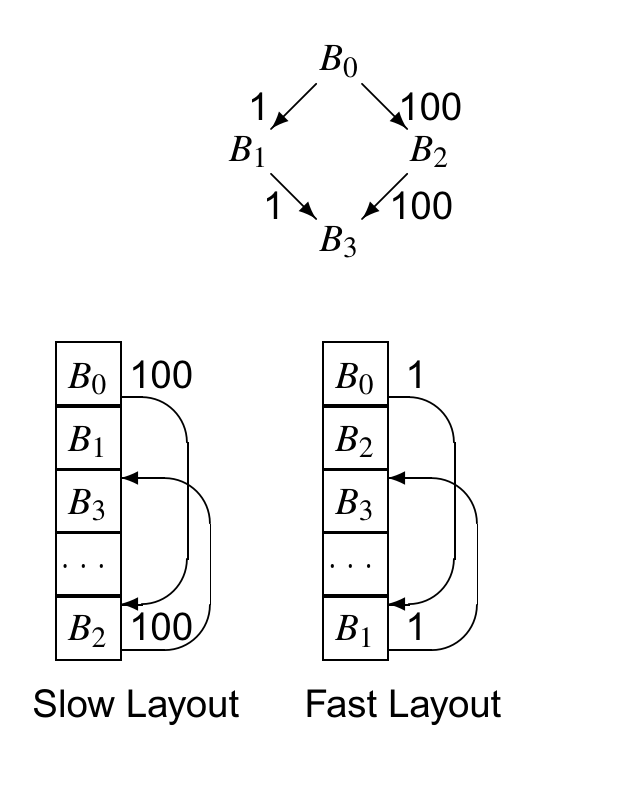
\includegraphics[width=0.31\textwidth]{images/layout_compare.png}
        \caption{两种不同布局的优劣\cite{cooper2011engineering}}
    \end{figure}

\end{frame}


\begin{frame}[fragile]
\frametitle{基本块放置 - Basic Block Placement}

    \begin{columns}
        \begin{column}{0.3\textwidth}
            \centering
            C Codes:
            \begin{lstlisting}
// hot path
if (cond)
    coldFunc();
// hot path again\end{lstlisting}
        \end{column}
        \begin{column}{0.65\textwidth}
            \begin{figure}
                \centering
                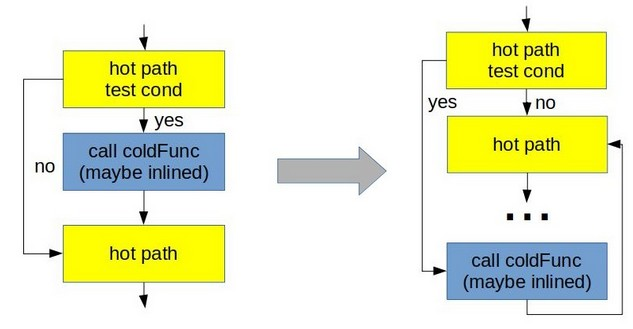
\includegraphics[width=1.\textwidth]{images/hot_cold_placement.jpg}
                \caption{布局优化示例}
            \end{figure}
        \end{column}
    \end{columns}
    \begin{itemize}
        \item 不进行分支跳转往往比跳转代价更低(maintain fall through)
        \item 更好地利用 Cache ($\mu$op-cache) (局部性)
    \end{itemize}

\end{frame}

\begin{frame}
\frametitle{基本块对齐 - Basic Block Alignment}
\centering

A brief explanation of the manner:

\begin{figure}
    \centering
    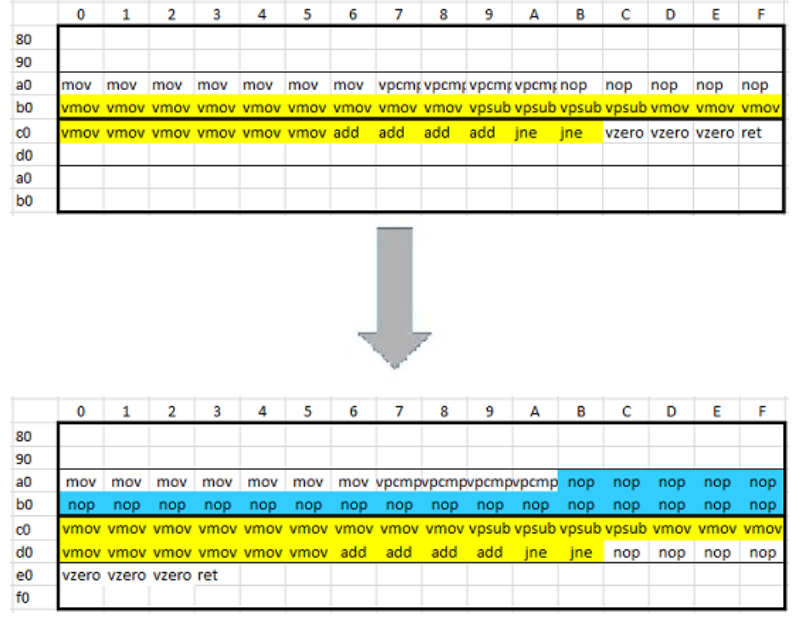
\includegraphics[width=0.618\textwidth]{images/alignment.png}
\end{figure}

\end{frame}
\begin{frame}[fragile]
    \frametitle{冷热代码分离 - 分离前}
    冷热代码分离的核心思想是,将冷代码(如错误处理)分成一个独立的函数调用,从原过程(procedure)中分离,然后用一个函数调用语句代替冷代码,从而提高热代码的连续性、局部性。
    \begin{columns}
        \begin{column}{0.7\textwidth}
            \begin{lstlisting}
void foo(bool cond1, bool cond2) {
    // hot path
    if (cond1)
        // cold code 1
    //hot code
    if (cond2)
        // cold code 2
}
            \end{lstlisting}
        \end{column}
    \end{columns}
\end{frame}


\begin{frame}[fragile]
    \frametitle{冷热代码分离 - 分离后的代码}
    \begin{columns}
        \begin{column}{1.0\textwidth}
            \begin{lstlisting}
void foo(bool cond1, bool cond2) {
    // hot path
    if (cond1)
        cold1(); 
    //hot code
    if (cond2)
        cold2(); 
    }
    
    void cold1() __attribute__((noinline)) { // cold code 1 }
    void cold2() __attribute__((noinline)) { // cold code 2 }
            \end{lstlisting}
        \end{column}
    \end{columns}
\end{frame}

\begin{frame}
    \frametitle{冷热代码分离 - 图}
这样做的好处是,热指令都会存在同一个cache line里,可以提高CPU前端数据结构的利用效率,例如I-cache 和 DSB-Cache
    \begin{figure}
        \centering
        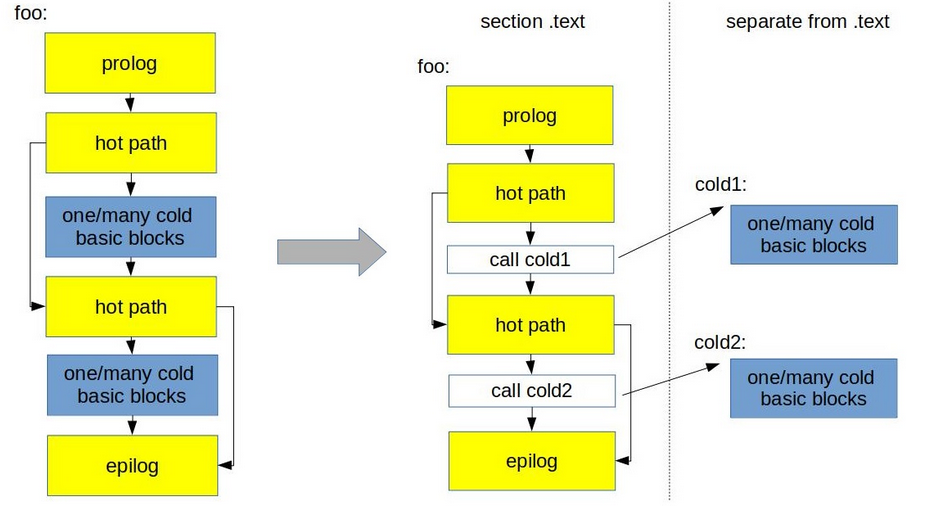
\includegraphics[width=0.68\textwidth]{images/splitting.png}
\caption{将冷代码过程转换为函数调用}
    \end{figure}

\end{frame}
\section{代码块放置(Block Placement)}

\begin{frame}
    \frametitle{控制流图链剖分}

    首先对CFG建立链剖分,建立的原则是,经常被执行的边被放在一起,形成一条链(Chain)。

    一条链包含一个或多个基本块(BB),并且每个路径都有一个优先级(priority)决定了他们在最终的代码布局中的情况。

    \begin{figure}
        \centering
        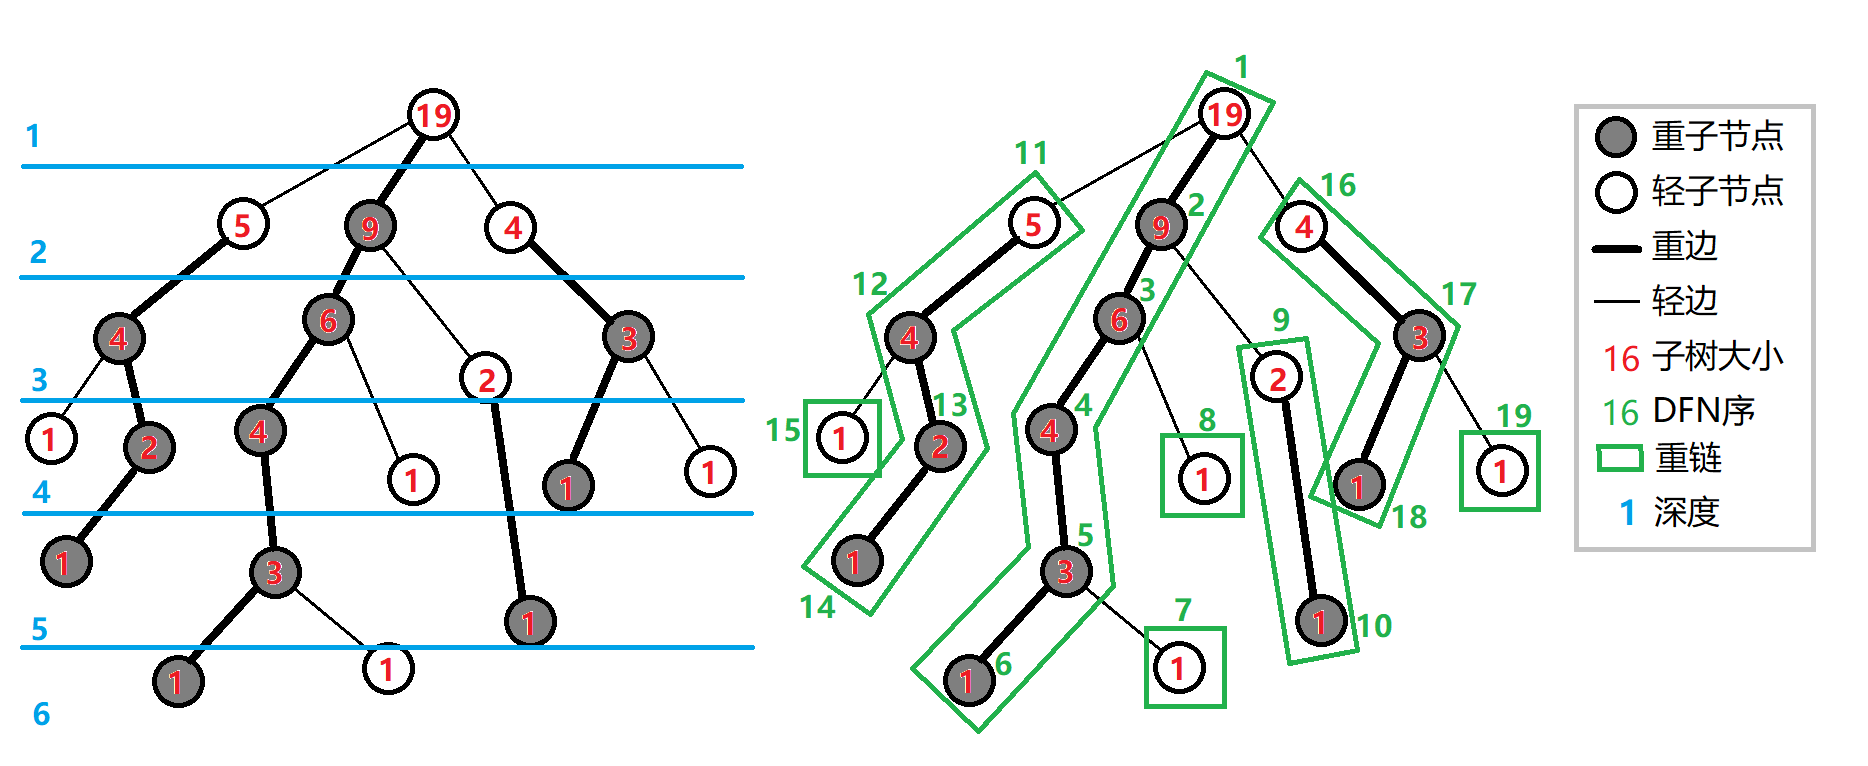
\includegraphics[width=0.7\textwidth]{images/hld.png}
        \caption{\cite{unknown-author-2022}轻重链剖分,树上链剖分的一种}
    \end{figure}

\end{frame}


\begin{frame}[fragile]
    \frametitle{Kruskal ? Prim ?}

    CFG没有树这么好的性质,CFG是一个有向图。构建链的方法是每次从边集合中选一条没有被选中的边(按照边的权重顺序),然后形成链状结构。

    \begin{figure}
        \centering
        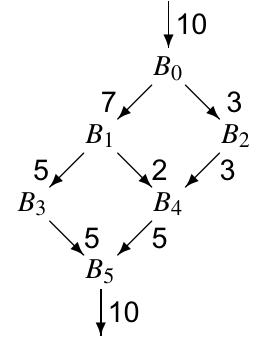
\includegraphics[width=0.3\textwidth]{images/example_cfg.png}
        \caption{CFG的一个例子\cite{cooper2011engineering}}
    \end{figure}



\end{frame}

\begin{frame}
    \frametitle{CFG上的贪心启发式链剖分 (Greedy heuristic chain div on CFGs)}

    \begin{algorithmic}
        \State $E$ $\gets$ | edges |
        \For{each block b}
        \State make a degenerate chain, $d$, for $b$
        \State priority($d$) $\gets$ $E$
        \EndFor
        \State $P \gets 0$
        \For{each CFG edge $<x, y>, x \neq y$, in decreasing freq order}
        \State $ t \gets $ priority($a$)
        \State append $b$ onto $a$
        \State priority($a$) $\gets$ $\min$ ($t$, priority($b$), $P$++)
        \EndFor
    \end{algorithmic}


\end{frame}

\begin{frame}
    \frametitle{CFG上的贪心启发式链剖分 (Greedy heuristic chain div on CFGs)}

    \begin{columns}
        \begin{column}{0.3\textwidth}
            \begin{figure}
                \centering
                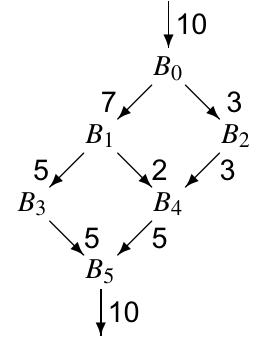
\includegraphics[width=1.0\textwidth]{images/example_cfg.png}
                \caption{CFG的一个例子\cite{cooper2011engineering}}
            \end{figure}
        \end{column}
        \begin{column}{0.6\textwidth}
            \begin{figure}
                \centering
                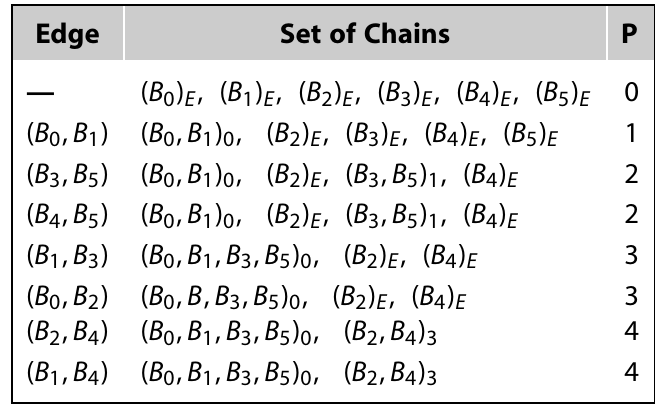
\includegraphics[width=1.0\textwidth]{images/greedy.png}
                \caption{算法每个过程选择的边,和对应的边集}
            \end{figure}
        \end{column}
    \end{columns}

\end{frame}


\begin{frame}
    \frametitle{基于WorkList组合最终的代码布局(Code Layout)}

    \begin{algorithmic}
        \State $t$ $\gets$ chain headed by the CFG entry node
\State $WorkList$ $\gets$ $\lbrace(t, priority(t))\rbrace$ $ \qquad \Leftarrow$ Heap\cite{forsythe1964algorithms}
        \While{$WorkList \neq \emptyset$}
        \State remove a chian $c$ of lowest priority from $WorkList$
        \For{each block $x$ in $c$ in chain}
        \State place $x$ and the end of assembly codes
        \EndFor
        \For{each block $x$ in $c$}
        \For{each edge $<x, y$ where $y$ is unplaced}
        \State $t \gets $ chain containing $<x, y>$
        \If{$(t, priority(t)) \notin WorkList$}
        $WorkList \gets WorkList \bigcup \lbrace (t, priority(t)) \rbrace$
        \EndIf
        \EndFor
        \EndFor
        \EndWhile
    \end{algorithmic}

\end{frame}


\begin{frame}
    \frametitle{Example}
    \begin{columns}
        \begin{column}{0.5\textwidth}
            \begin{figure}
                \centering
                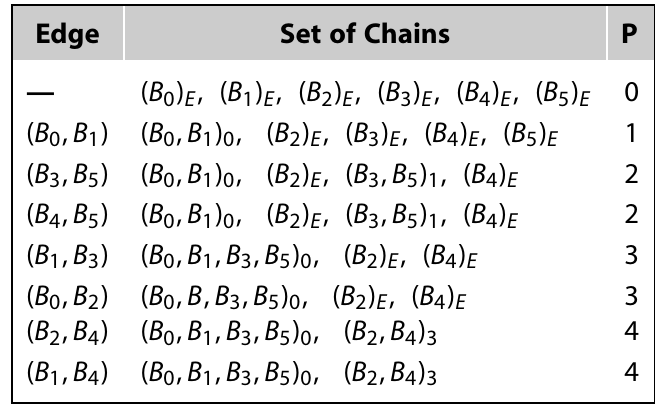
\includegraphics[width=1.0\textwidth]{images/greedy.png}
                \caption{上一个过程形成的链}
            \end{figure}
        \end{column}
        \begin{column}{0.5\textwidth}
            \begin{figure}
                \centering
                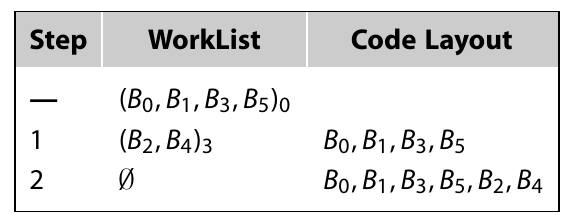
\includegraphics[width=1.0\textwidth]{images/worklist.png}
                \caption{生成最终的代码布局}
            \end{figure}
        \end{column}
    \end{columns}
\end{frame}
\section{LLVM 中如何实现这个算法}


\begin{frame}
    \frametitle{TL; DR}

    算法主体主要实现在 lib/CodeGen/MachineBlockPlacement.cpp

    \vspace{1.5em}

    其中分支概率等信息来源于 Block\{Frequency, ProbabilityInfo\}

    \vspace{1.5em}

    各个 Target 需要实现 \{ analyze, insert, remove \}Branch等虚函数,RISC-V在 5 年前,D40808
    \cite{llvmriscvimplbranchanalysis2022}实现。
    \begin{table}
        \begin{tabular}{ccc}
            \toprule
            功能     & 实现                  & 源代码位置                                                                         \\
            \midrule
            边权     & BlockFrequency        & \cite{llvmblockfreqinfoimpl2022}                                                   \\
            块放置   & MachineBlockPlacement & buildCFGChains()\cite{llvmmachineblockplacement2022}                               \\
            块对齐   & MachineBlockPlacement & alignBlocks()\cite{llvmmachineblockplacement2022}                                  \\
            分支分析 & RISCVInstrInfo        & analyzeBranch()\cite{llvmriscvinstrinfo2022}\cite{llvmriscvimplbranchanalysis2022} \\
            \bottomrule
        \end{tabular}
        \caption{各个功能的实现情况和所在的位置}
    \end{table}

\end{frame}
\section{References}


\begin{frame}[allowframebreaks]
    \frametitle{References}
    \bibliographystyle{ieeetr}
    \bibliography{main.bib}
\end{frame}
\end{document}